\documentclass[conference]{IEEEtran}

\usepackage[T1]{fontenc}
\usepackage[utf8]{inputenc}
\usepackage[brazilian]{babel}
\usepackage{cite}
\usepackage{graphicx}
\usepackage{url}
\usepackage{microtype}
\usepackage[hidelinks]{hyperref}

\graphicspath{{figures/}}
\renewcommand{\abstractname}{Resumo}
\renewcommand{\IEEEkeywordsname}{Palavras-chave}
\addto\captionsbrazilian{\renewcommand{\figurename}{Fig.}}

\begin{document}

\title{Aplicação de Redes de Sensores Sem Fio na Agricultura de Precisão: Monitoramento de Umidade do Solo}

\author{%
\IEEEauthorblockN{Edson Claiton da Silva Júnior}
\IEEEauthorblockA{Mestrado em Telecomunicações\\
Instituto Nacional de Telecomunicações (INATEL)\\
Santa Rita do Sapucaí, MG, Brasil\\
edson.silva@mtel.inatel.br}}

\maketitle

\begin{abstract}
A agricultura de precisão tem se destacado como uma importante estratégia para aumentar a eficiência no uso dos recursos hídricos e melhorar a produtividade agrícola. Nesse contexto, as Redes de Sensores Sem Fio (RSSF/WSN) possibilitam o monitoramento contínuo de variáveis ambientais e da umidade do solo por meio de sensores distribuídos em campo e interligados por tecnologias de comunicação sem fio. Este trabalho apresenta uma abordagem sobre a aplicação de RSSF no monitoramento da umidade do solo, abrangendo os principais conceitos relacionados às redes de sensores, os tipos de sensores empregados, como FDR, TDR e RFID, e as tecnologias de comunicação ZigBee, Bluetooth Low Energy e LoRaWAN. Além disso, são discutidas as características, vantagens e desafios da utilização dessas tecnologias em sistemas de agricultura de precisão. Os resultados demonstram que a adoção de RSSF contribui para o gerenciamento eficiente da irrigação e para a redução do desperdício de água.
\end{abstract}

\begin{IEEEkeywords}
agricultura de precisão, Internet das Coisas, LoRaWAN, monitoramento inteligente, redes de sensores sem fio, umidade do solo.
\end{IEEEkeywords}

\section{Introdução}

Nas últimas décadas, a utilização de água na agricultura tornou-se objeto de preocupação para a Organização das Nações Unidas para a Alimentação e a Agricultura (FAO). Carlesso \emph{et al.} estimaram em torno de 300 milhões de hectares de áreas irrigadas \cite{carlesso2009}. Estudos apontam que a agricultura consome aproximadamente 70\% da água disponível mundialmente para a produção agrícola \cite{hardie2020}.

As tendências de escassez hídrica indicam que, até 2030, pode ocorrer um aumento de até 2.000\% em relação aos últimos 100 anos, constituindo um cenário que demanda o gerenciamento eficiente dos recursos \cite{silva2024}.

Nessa conjuntura, métricas e sistemas de monitoramento inteligente oferecem formas eficazes de acompanhar e controlar a umidade do solo. Uma irrigação precisa permite aplicar a quantidade de água adequada a determinada área, evitando desperdícios e mantendo condições propícias ao plantio \cite{silva2024}.

As redes de sensores sem fio vêm se consolidando ao longo dos anos. Seu objetivo é reunir um grande conjunto de nós sensores capazes de se interconectar e formar uma malha inteligente \cite{gta2002}.

Considerando que a escassez de água pode se tornar um problema em um futuro próximo e que a agricultura depende desse recurso, as redes de sensores sem fio aplicadas ao monitoramento da umidade do solo contribuem para a otimização do uso da água e para o gerenciamento das condições do solo.

\section{Fundamentação Teórica}

As redes de sensores sem fio (RSSF/WSN) possuem particularidades em comparação com redes convencionais de computadores e dispositivos, principalmente em razão de fatores como consumo de energia, tamanho, comunicação e possibilidade de falhas. Os nós sensores comunicam-se entre si e, diante de uma falha decorrente do esgotamento de energia, da perda de pacotes ou da indisponibilidade de um nó responsável por retransmitir informações, a fidelidade do sensoriamento pode ser prejudicada \cite{loureiro2003}.

Uma RSSF é composta por sensores de baixo consumo e baixo custo, mantendo capacidade de processamento e sensoriamento. Esses dispositivos são capazes de se comunicar sem fio em curtas distâncias e atuar de forma colaborativa com outros nós \cite{akyildiz2002}.

Os nós de uma rede de sensores podem ser distribuídos em determinada área sem a necessidade de uma localização previamente definida. Ao transmitirem os dados, os sensores também podem informar a localização do nó \cite{akyildiz2002}.

Um dos fatores que diferenciam os nós sensores dos dispositivos convencionais é o consumo energético. Nos nós, é necessário preservar a energia disponível e gerenciar o consumo. Em contrapartida, dispositivos convencionais costumam estar conectados a uma fonte fixa de energia e, portanto, não enfrentam a mesma restrição \cite{akyildiz2002}.

Em algumas topologias, os nós sensores atuam como repetidores das informações provenientes de outros nós, o que pode tornar o consumo da bateria maior do que o de sensores mais distantes das rotas principais \cite{akyildiz2002}.

As aplicações de redes de sensores podem abranger medições de temperatura, umidade, movimento veicular, luminosidade, pressão e ruído, entre outras grandezas. Os nós são desenvolvidos para realizar o sensoriamento, processar os dados e transmiti-los a outros nós \cite{akyildiz2002}.

\section{Redes de Sensores Sem Fio na Agricultura}

Os sensores FDR (\emph{Frequency Domain Reflectometry}) representam uma alternativa de menor custo para o monitoramento da umidade do solo. Esses sensores mensuram a quantidade de água presente no solo por meio da variação da constante dielétrica, possibilitando ampla utilização em sistemas de agricultura de precisão. Embora apresentem menor custo, podem sofrer influência das características físicas e químicas do solo, sendo necessárias calibrações adequadas para aumentar a acurácia das medições e a confiabilidade dos resultados \cite{hardie2020}.

Em aplicações que exigem maior confiabilidade, podem ser empregados sensores TDR (\emph{Time Domain Reflectometry}), amplamente reconhecidos pela elevada precisão na medição da umidade do solo. Seu princípio de funcionamento baseia-se na propagação de pulsos eletromagnéticos ao longo de sondas inseridas no solo, permitindo estimar o teor de água com alta confiabilidade. Entretanto, seu custo de aquisição é relativamente elevado quando comparado ao dos sensores FDR, o que pode inviabilizar sua utilização em aplicações agrícolas de larga escala \cite{hardie2020}.

Tecnologias de sensores baseadas em RFID constituem alternativas ainda em estudo para o monitoramento da umidade do solo. Elas apresentam baixo custo e podem funcionar sem baterias, utilizando a energia fornecida pelo dispositivo leitor. Entretanto, o alcance é reduzido e a extração dos dados requer pequena distância entre o sensor e o leitor, o que ainda restringe sua aplicação em áreas agrícolas extensas \cite{hardie2020}.

\section{Tecnologias de Comunicação}

A comunicação é um elemento essencial dos nós sensores, pois, após a coleta e o processamento da grandeza, os dados precisam ser enviados a um destino. A transmissão de dados é responsável por uma parcela significativa do consumo de energia de um nó e, em geral, demanda mais energia do que a recepção \cite{akyildiz2002}.

A Fig.~\ref{fig:protocol-stack} apresenta a arquitetura do protocolo de comunicação descrita por Akyildiz \emph{et al.}, composta pelas camadas de aplicação, transporte, rede, enlace de dados e física, além dos planos de gerenciamento de energia, mobilidade e tarefas \cite{akyildiz2002}.

\begin{figure}[!t]
  \centering
  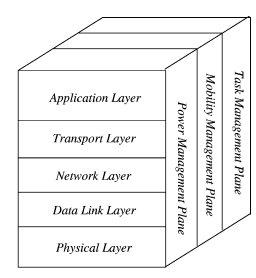
\includegraphics[width=0.62\columnwidth]{image1.png}
  \caption{Arquitetura do protocolo de comunicação em RSSF. Fonte: adaptado de \cite{akyildiz2002}.}
  \label{fig:protocol-stack}
\end{figure}

Segundo Yick \emph{et al.}, a implementação dos protocolos nas diferentes camadas impacta significativamente o consumo de energia, a eficiência do sistema e a latência \cite{yick2008}. Os desafios de uma rede de sensores incluem a obtenção de hardware de baixo custo e baixo consumo, capaz de proporcionar longa duração da bateria sem comprometer o processamento e a transmissão dos dados \cite{akyildiz2002}.

Nas últimas décadas, foram desenvolvidas aplicações de redes de sensores em ambientes subterrâneos, terrestres, subaquáticos, móveis e multimídia \cite{yick2008}. Na agricultura, o uso de fertilizantes sintéticos requer automação e tecnologias que apoiem a produção de precisão \cite{zhang2002}.

O conceito de agricultura de precisão consiste em um sistema que busca alta eficiência, baixo uso de insumos e sustentabilidade, utilizando tecnologias como sistemas de posicionamento global (GPS), sistemas de informação geográfica, controle automatizado, sensoriamento remoto, processamento de informações e telecomunicações \cite{zhang2002}.

As RSSF estão presentes na agricultura em aplicações como a medição de nutrientes para avaliação da qualidade do solo e o sensoriamento da irrigação para mapeamento da umidade e das condições meteorológicas \cite{ojha2015}. A atenuação dos sinais e a baixa eficiência energética podem ocorrer dependendo das condições de instalação dos nós e do tempo de utilização da comunicação, reduzindo a vida útil da bateria \cite{ojha2015}.

A Fig.~\ref{fig:above-ground} apresenta uma distribuição de nós sensores sobre o solo, que se comunicam entre si e encaminham as informações ao \emph{gateway} principal para posterior transmissão dos dados à nuvem.

\begin{figure}[!t]
  \centering
  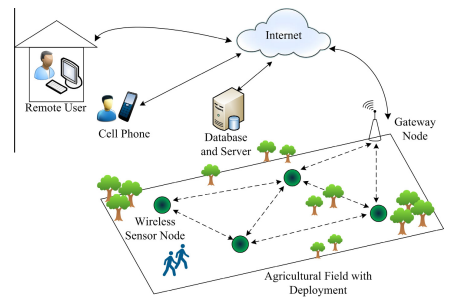
\includegraphics[width=\columnwidth]{image2.png}
  \caption{Arquitetura de sensores sobre o solo. Fonte: adaptado de \cite{ojha2015}.}
  \label{fig:above-ground}
\end{figure}

A Fig.~\ref{fig:underground} apresenta uma aplicação de nós sensores no subsolo. Suas particularidades estendem-se além da disposição física: as dificuldades incluem a atenuação severa do sinal e a necessidade de mais nós e \emph{gateways} do que na arquitetura da Fig.~\ref{fig:above-ground}. A perda significativa de sinal também compromete a vida útil da bateria. Para obter comunicação eficaz, utiliza-se um \emph{gateway} no subsolo, que se comunica com os demais nós sensores, e outro sobre o solo, responsável por retransmitir as informações para a nuvem \cite{akyildiz2002}.

\begin{figure}[!t]
  \centering
  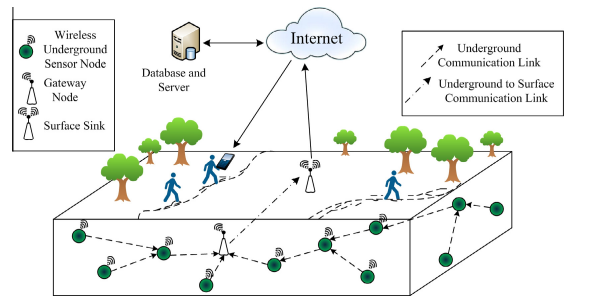
\includegraphics[width=\columnwidth]{image3.png}
  \caption{Arquitetura de sensores em ambiente subterrâneo. Fonte: adaptado de \cite{ojha2015}.}
  \label{fig:underground}
\end{figure}

Os sistemas de monitoramento da irrigação proporcionam melhor gerenciamento e aproveitamento da água nas propriedades rurais. Os nós sensores podem atuar em sistemas de microirrigação, favorecendo a eficiência e a redução de custos \cite{ojha2015}.

O objetivo da Internet das Coisas (IoT) é promover a interconexão e a comunicação entre dispositivos, incluindo atuadores e sensores incorporados a sistemas de telecomunicações. A conexão desses dispositivos à Internet possibilita a comunicação entre equipamentos e a interação humana com eles \cite{centenaro2016}.

Os protocolos ZigBee e Bluetooth vêm sendo utilizados há anos e permanecem como alternativas viáveis devido ao baixo consumo, uma característica essencial para dispositivos de IoT. Em contrapartida, suas limitações incluem a cobertura em áreas urbanas e extensas \cite{centenaro2016}.

Entre as tecnologias empregadas em RSSF destaca-se o ZigBee, baseado no padrão IEEE~802.15.4. Essa tecnologia apresenta baixo consumo de energia e permite a formação de redes em malha, nas quais os nós sensores podem retransmitir informações entre si. A topologia oferece flexibilidade para expandir a cobertura da rede, mas requer mecanismos adicionais de roteamento e manutenção das rotas de comunicação, o que pode aumentar o tráfego de controle e afetar a eficiência em grandes áreas agrícolas.

O Bluetooth Low Energy (BLE), utilizado em aplicações de IoT, diferencia-se pela redução do consumo de energia, aumentando a autonomia de dispositivos alimentados por baterias. Suas limitações de alcance, porém, podem inviabilizar o uso em aplicações agrícolas de grande porte; por isso, é mais adequado para estufas, laboratórios agrícolas ou monitoramento localizado \cite{centenaro2016}.

Centenaro \emph{et al.} destacam a rede LoRa como uma tecnologia LPWAN (\emph{Low-Power Wide-Area Network}) desenvolvida para aplicações de longa distância e baixo consumo de energia. A cobertura de uma LPWAN pode alcançar de 10 a 15~km em áreas rurais, enquanto, em zonas urbanas, o alcance decai para 3 a 5~km. O LoRaWAN emprega a topologia estrela de estrelas apresentada na Fig.~\ref{fig:lorawan} \cite{centenaro2016}.

\begin{figure}[!t]
  \centering
  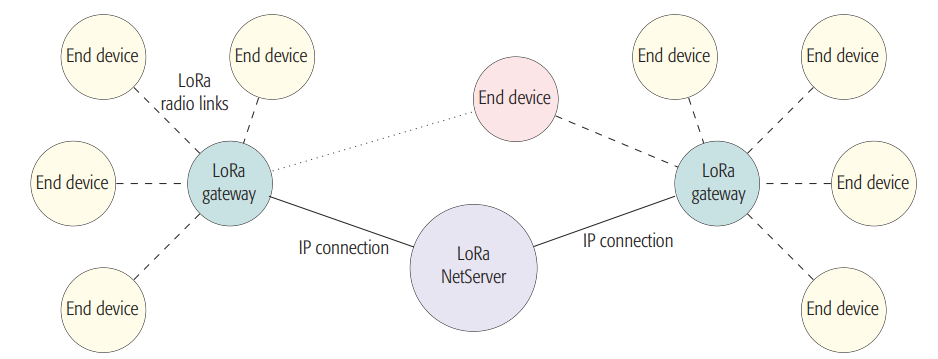
\includegraphics[width=\columnwidth]{image4.png}
  \caption{Arquitetura estrela de estrelas utilizada pelo LoRaWAN. Fonte: adaptado de \cite{centenaro2016}.}
  \label{fig:lorawan}
\end{figure}

Em aplicações agrícolas que envolvem grandes áreas de cultivo, o LoRaWAN torna-se uma alternativa interessante. Essa tecnologia pertence à categoria LPWAN, caracterizada por longas distâncias de comunicação e baixo consumo energético. Ao contrário das redes em malha, o LoRaWAN utiliza uma topologia em estrela, na qual os nós sensores enviam as medições diretamente ao \emph{gateway}. Essa organização reduz a complexidade da rede e facilita a implementação de sistemas de monitoramento da umidade do solo, da temperatura e das condições ambientais em propriedades rurais extensas \cite{centenaro2016}.

\section{Conclusão}

ZigBee e Bluetooth Low Energy são amplamente empregados em aplicações de redes de sensores sem fio. O protocolo LoRaWAN, por sua vez, apresenta vantagens significativas para ambientes agrícolas devido ao maior alcance de comunicação, à menor necessidade de infraestrutura intermediária e ao baixo consumo energético. Essas características são essenciais para o monitoramento de grandes áreas rurais.

\begin{thebibliography}{10}

\bibitem{carlesso2009}
R. Carlesso, M. T. Petry, and C. Trois, ``The use of a meteorological station network to provide crop water requirement information for irrigation management,'' in \emph{Proc. IFIP}, vol. 293, pp. 19--27, 2009, doi: 10.1007/978-1-4419-0209-2\_3.

\bibitem{hardie2020}
M. Hardie, ``Review of novel and emerging proximal soil moisture sensors for use in agriculture,'' \emph{Sensors}, vol. 20, no. 23, Art. no. 6934, 2020, doi: 10.3390/s20236934.

\bibitem{silva2024}
A. C. Silva \emph{et al.}, ``Plataforma digital integrada a rede de sensores sem fio para monitoramento contínuo da umidade do solo,'' in \emph{Proc. WCAMA}, 2024. [Online]. Available: \href{https://sol.sbc.org.br/index.php/wcama/article/view/29431}{SBC OpenLib}.

\bibitem{gta2002}
GTA/UFRJ, ``Redes de sensores sem fio.'' [Online]. Available: \href{https://www.gta.ufrj.br/grad/02_2/Redes%20de%20sensores/Redes%20de%20Sensores%20Sem-fio.doc}{GTA/UFRJ}. Accessed: Aug. 20, 2026.

\bibitem{loureiro2003}
A. Loureiro \emph{et al.}, ``Redes de sensores sem fio.'' [Online]. Available: \href{https://www.sensornet.dcc.ufmg.br/pdf/179_Loureiro_Nogueira_Ruiz_Mini_Nakamura_Figueiredo.pdf}{SensorNet/UFMG}. Accessed: Aug. 20, 2026.

\bibitem{akyildiz2002}
I. F. Akyildiz, W. Su, Y. Sankarasubramaniam, and E. Cayirci, ``Wireless sensor networks: A survey,'' \emph{Comput. Netw.}, vol. 38, no. 4, pp. 393--422, 2002, doi: 10.1016/S1389-1286(01)00302-4.

\bibitem{yick2008}
J. Yick, B. Mukherjee, and D. Ghosal, ``Wireless sensor network survey,'' \emph{Comput. Netw.}, vol. 52, no. 12, pp. 2292--2330, 2008, doi: 10.1016/j.comnet.2008.04.002.

\bibitem{zhang2002}
N. Zhang, M. Wang, and N. Wang, ``Precision agriculture: A worldwide overview,'' \emph{Comput. Electron. Agric.}, vol. 36, pp. 113--132, 2002, doi: 10.1016/S0168-1699(02)00096-0.

\bibitem{ojha2015}
T. Ojha, S. Misra, and N. S. Raghuwanshi, ``Wireless sensor networks for agriculture: The state-of-the-art in practice and future challenges,'' \emph{Comput. Electron. Agric.}, vol. 118, pp. 66--84, 2015, doi: 10.1016/j.compag.2015.08.011.

\bibitem{centenaro2016}
M. Centenaro, L. Vangelista, A. Zanella, and M. Zorzi, ``Long-range communications in unlicensed bands: The rising stars in the IoT and smart city scenarios,'' \emph{IEEE Wireless Commun.}, vol. 23, no. 5, pp. 60--67, Oct. 2016, doi: 10.1109/MWC.2016.7721743.

\end{thebibliography}

\end{document}
